\documentclass[17pt, t, lualatex]{beamer}



\title{Hidrodinámica del Río Magdalena a la altura de Barrancabermeja}
\date{\today}
\institute[UJTL]{Universidad Jorge Tadeo Lozano}
\author{Ludwig Alvarado Becerra}

\usepackage{amsmath, amssymb, mathtools}
\usepackage[spanish]{babel}
\usepackage{biblatex}
\usepackage{hyperref}
\usepackage{xurl}
\usepackage{svg}

\addbibresource{referencias.bib}  % Make sure your .bib file is correctly named


\addbibresource{referencias.bib}

% Probably load as late as possible
% Other options are
% - engine=pdflatex to compile in pdfLaTeX (with different fonts),
% - mathshape=rm to use serif font for math,
% - mathsahpe=custom to not set any math font (so that you can define your own math fonts)
\usetheme[engine=lualatex, mathshape=sf, fontdir=kthpq-files/fonts/Figtree/]{kthpq}
\setmonofont{Bitstream Vera Sans Mono}[Scale=.9]

% Custom colors (see beamercolorthemecustom.sty for more details)
% \usecolortheme{custom}

% Modify the headline template: KTH-full, KTH-section-only, or KTH-frametitle-only.
% \setbeamertemplate{headline}[KTH-full]

% Custom footline
% \setfootline{left}{center}{right}

\begin{document}

\inserttitlepage

\section{Exploración de datos}

\insertsectionpage

\begin{frame}[allowframebreaks]
  \frametitle{Exploración de datos}
  De acuerdo a Deaton\cite{deaton1999dynamic} la disponibilidad de los siguientes datos es crucial:

  \begin{itemize}
    \item Características topográficas del canal:
          \begin{itemize}
            \item Longitud.
            \item Elevación.
            \item Pendientes,
          \end{itemize}
    \item Características de transporte del canal:
          \begin{itemize}
            \item Elevación de la superficie del agua.
            \item Ancho.
            \item Coeficientes de rugosidad.
          \end{itemize}
    \item Datos de la condición final de frontera.
    \item Condición inicial.
  \end{itemize}

\end{frame}

\begin{frame}[allowframebreaks]
  \frametitle{Región de estudio}
  
  \begin{figure}[ht]
    \centering
    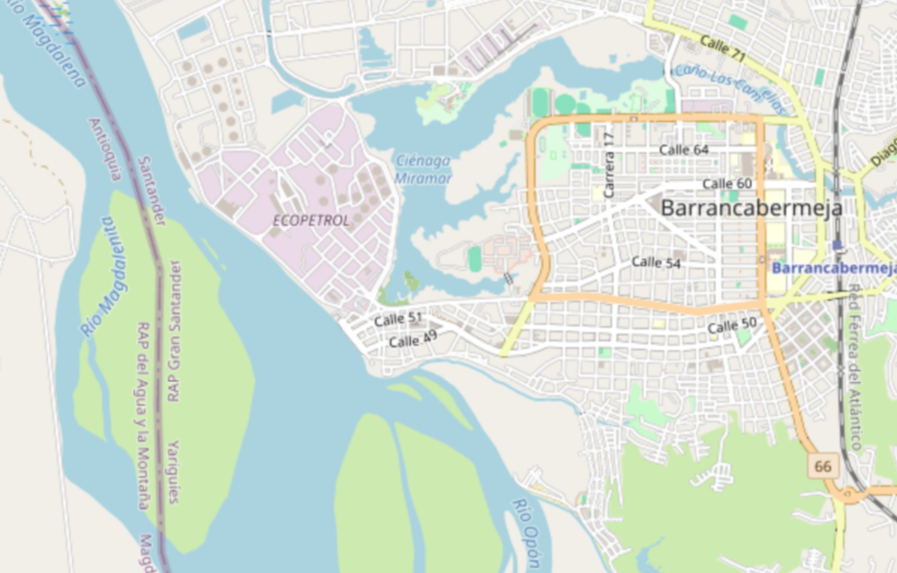
\includegraphics[width=0.5\textwidth]{img/OSM-1.png}
    \caption{Región a estudiar del Río Magdalena. Datos de \textit{OpenStreetMap} (OSM)\cite{openstreetmap_magdalena2025}}
  \end{figure}

  \begin{figure}[ht]
    \centering
    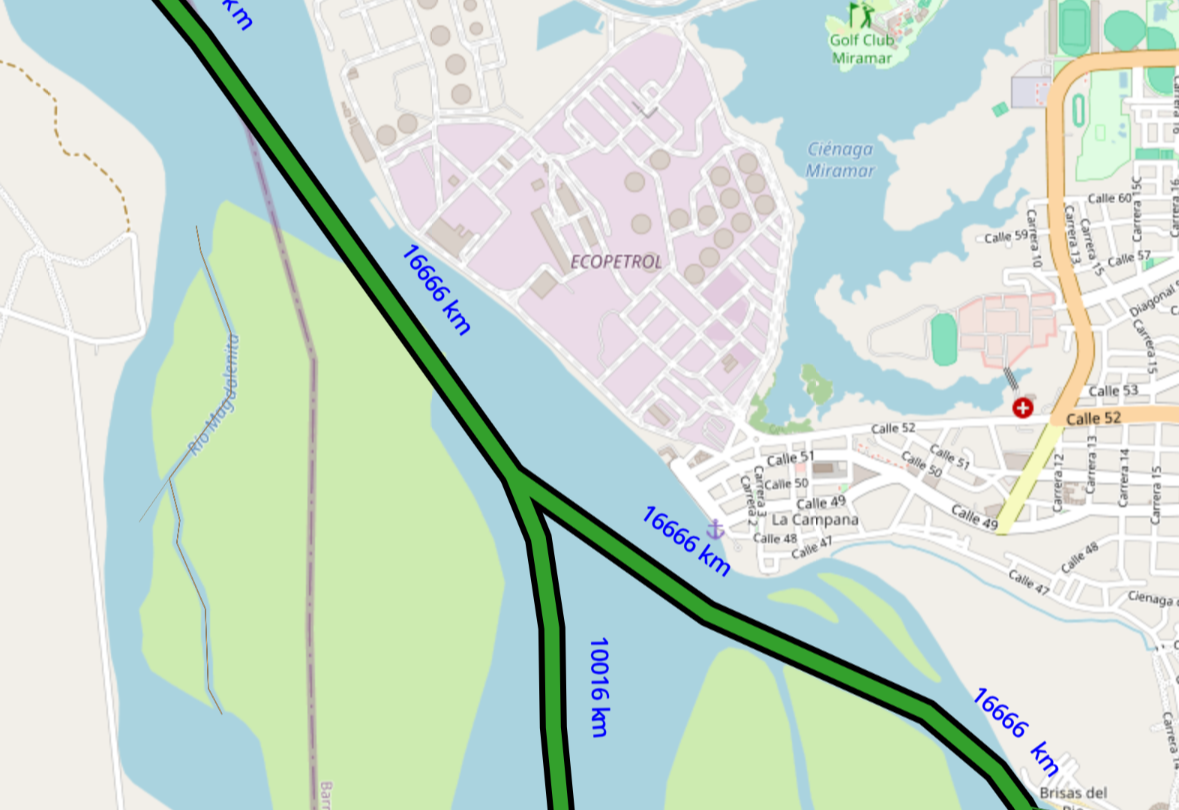
\includegraphics[width=0.5\textwidth]{img/Waterway.png}
    \caption{Río Magdalena. Datos sacados de \textit{Waterway}\cite{waterwaymap2025}}
  \end{figure}

  \begin{figure}[ht]
    \centering
    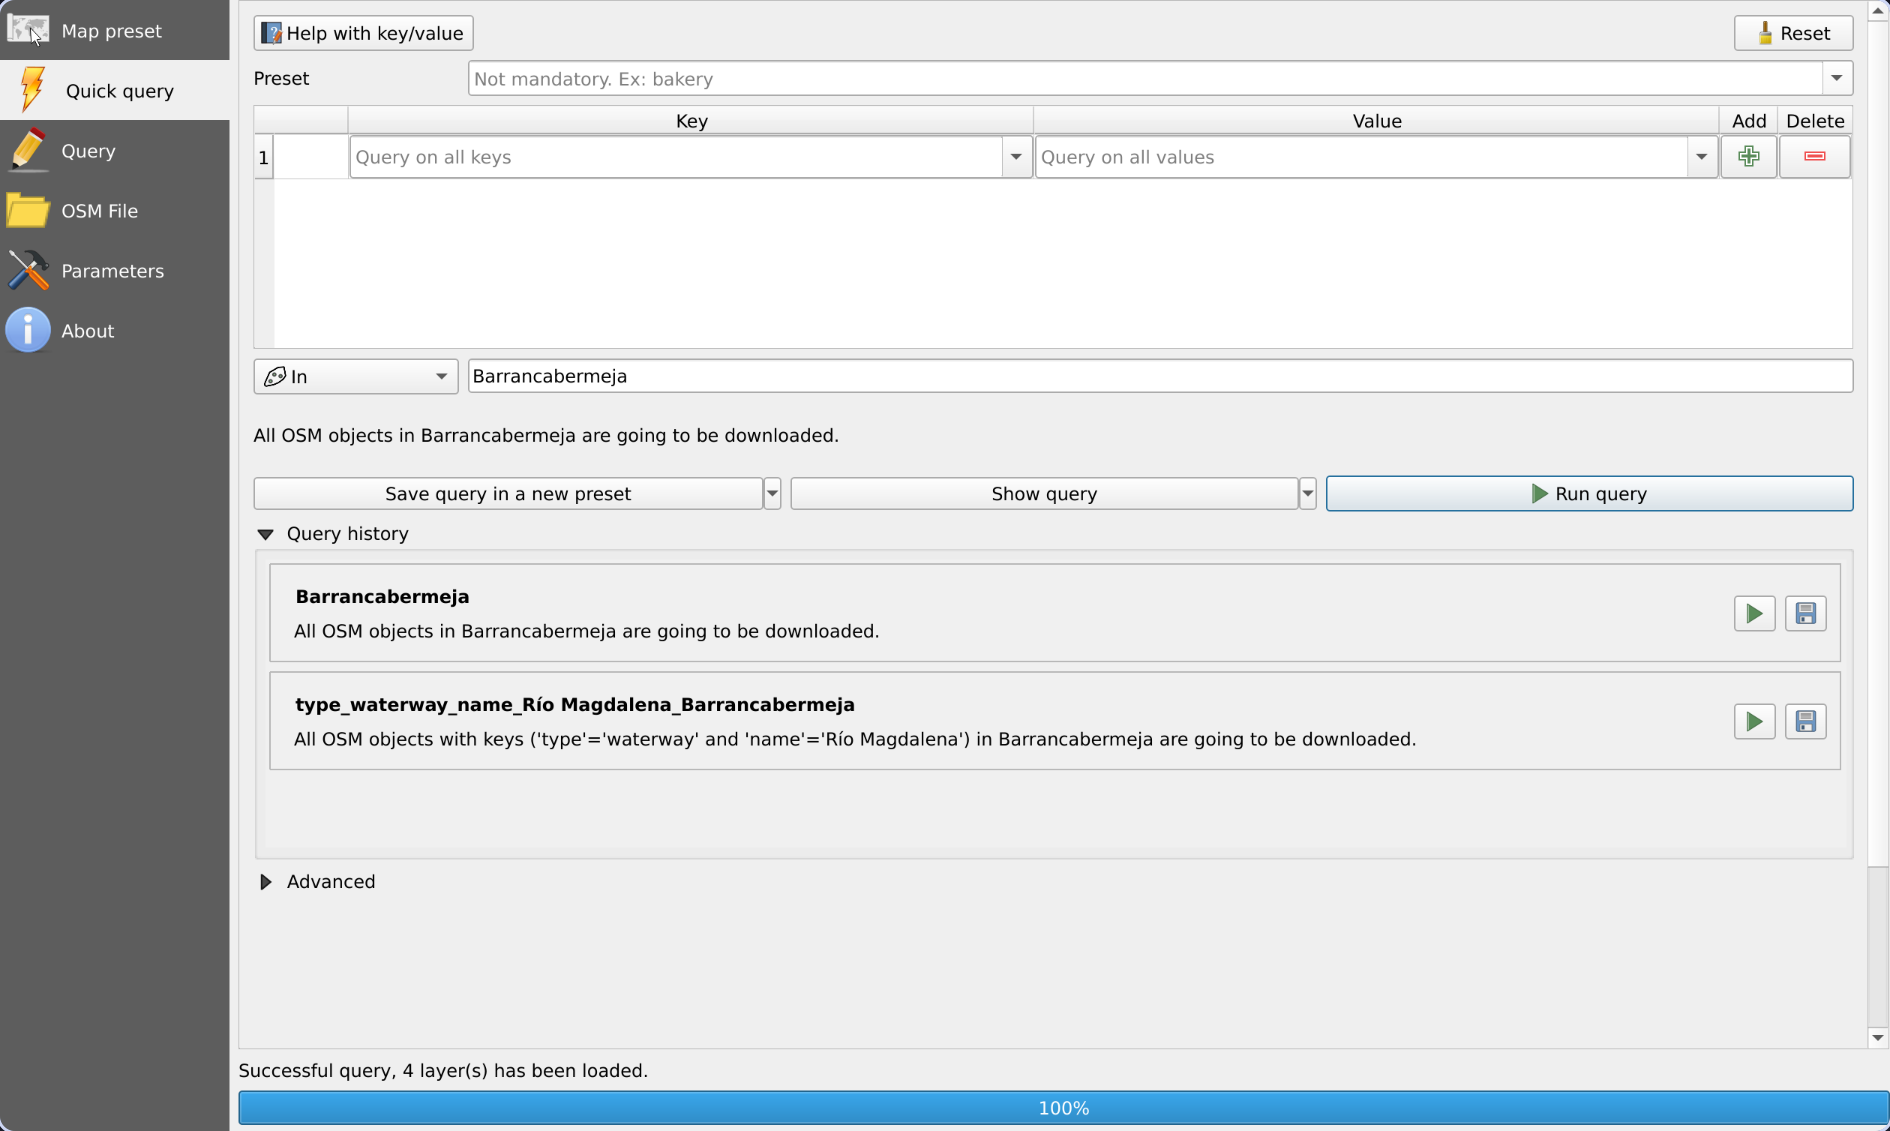
\includegraphics[width=0.5\textwidth]{img/QGIS-5.png}
    \caption{Consulta de datos utilizando QuickOSM\cite{quickosm2025}}
  \end{figure}


  \begin{figure}[ht]
    \centering
    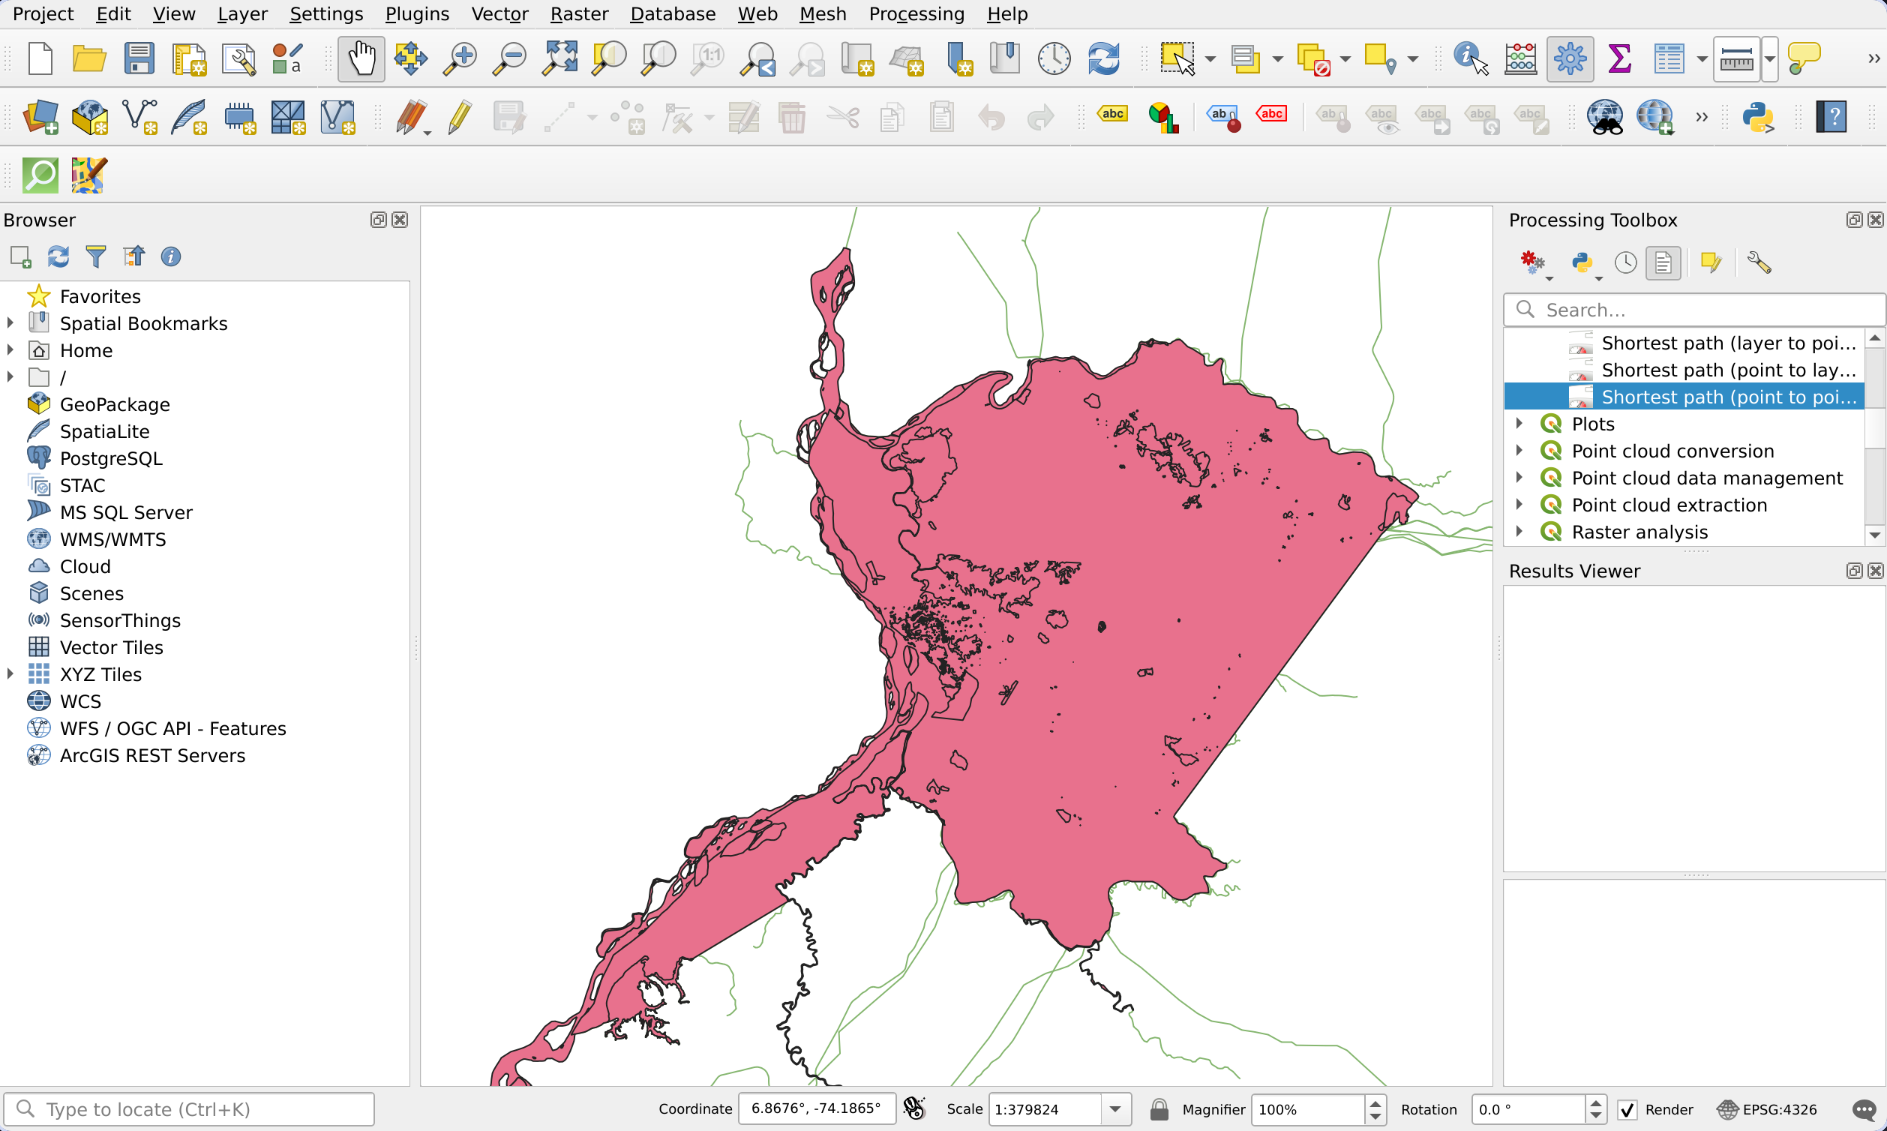
\includegraphics[width=0.55\textwidth]{img/QGIS-1.png}
    \caption{Región de Barrancabermeja, elaboración propia en QGIS\cite{qgis2025}, datos de OSM\cite{openstreetmap_magdalena2025}.}
  \end{figure}


  \begin{columns}
    \begin{column}{.3\textwidth}
      \begin{itemize}
        \item Se filtra la capa del Río Magdalena y se le cambia el color para que destaque.
      \end{itemize}
    \end{column}

    \begin{column}{.7\textwidth}
      \begin{figure}[ht]
        \centering
        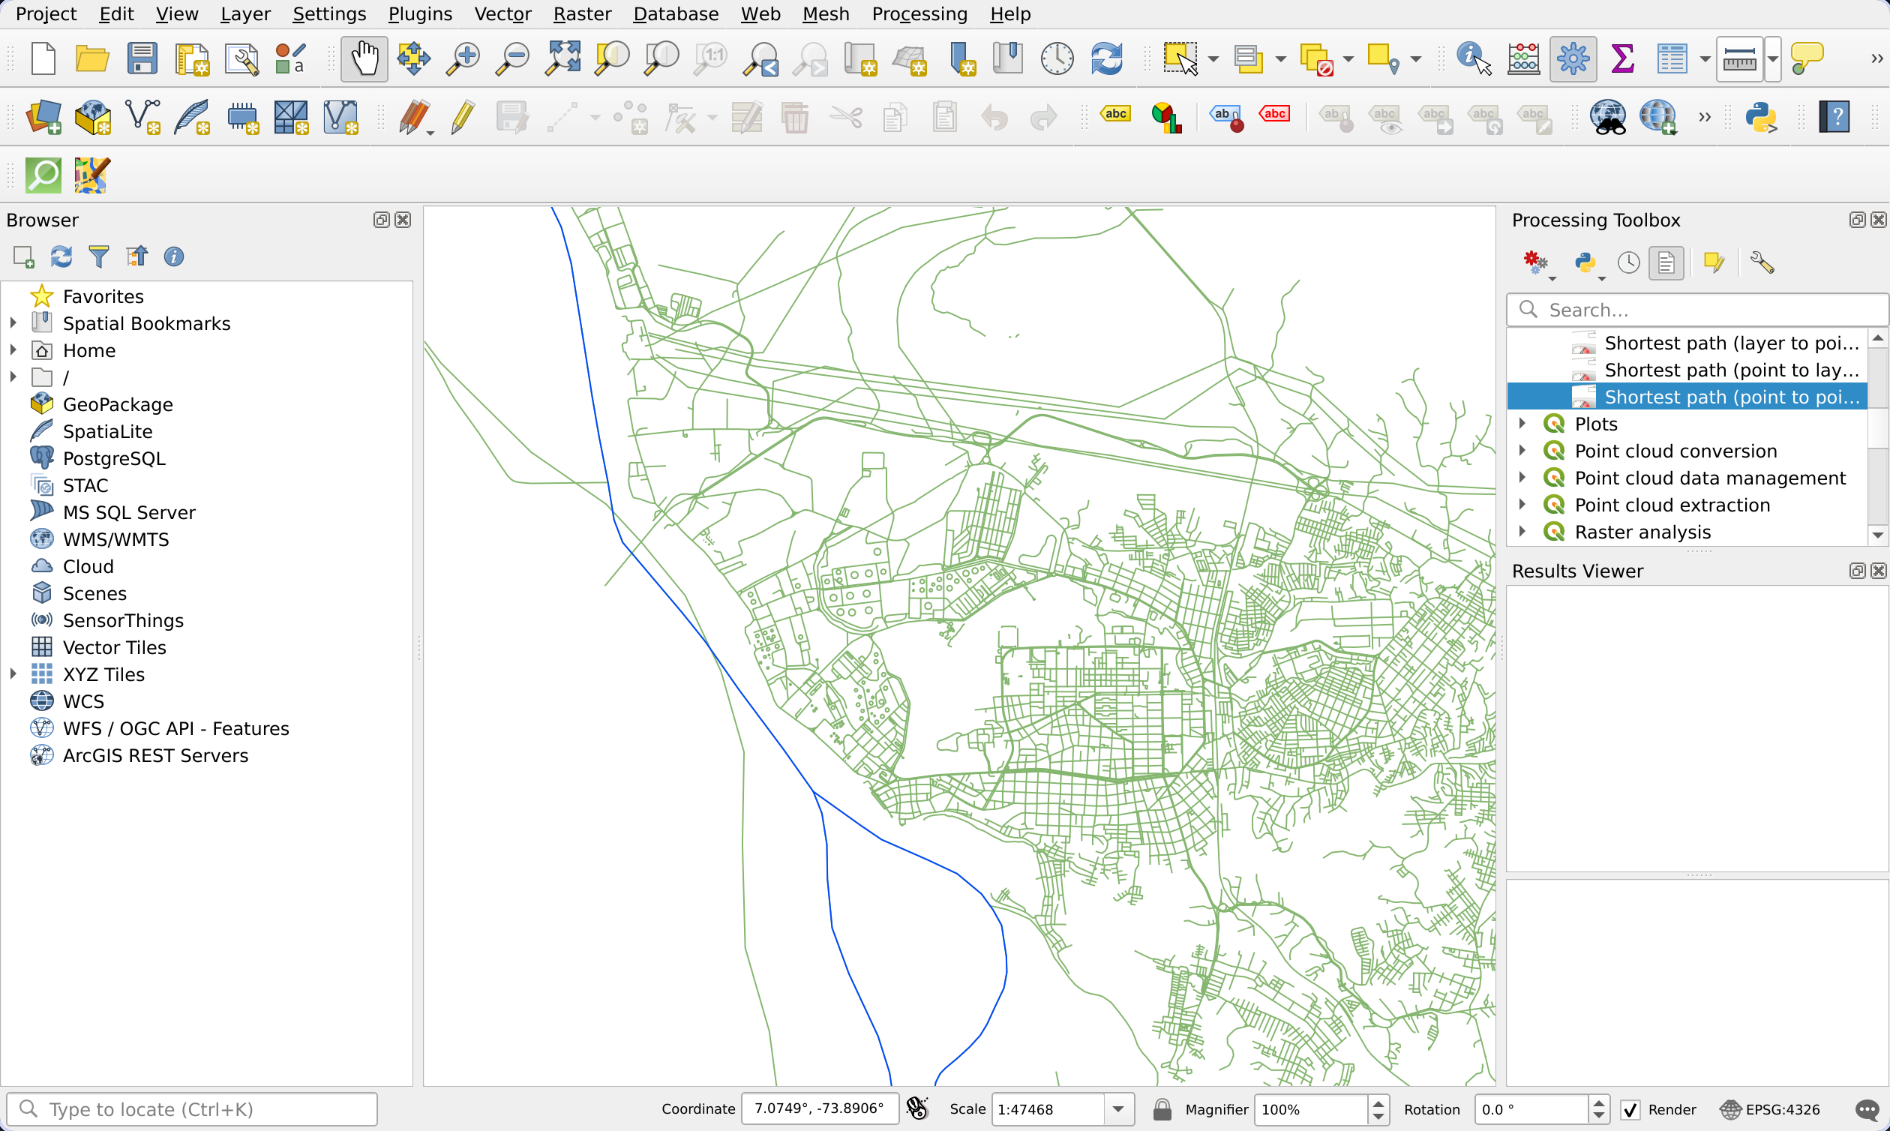
\includegraphics[width=0.8\textwidth]{img/QGIS-2.png}
        \caption{Elaboración propia.}
      \end{figure}
    \end{column}
  \end{columns}


  \begin{columns}
    \begin{column}{.3\textwidth}
      \begin{itemize}
        \item Utilizar \texttt{Vector} > \texttt{Geometry Tools} > \texttt{Extract Vertices...}
      \end{itemize}
    \end{column}

    \begin{column}{.7\textwidth}
      \begin{figure}[ht]
        \centering
        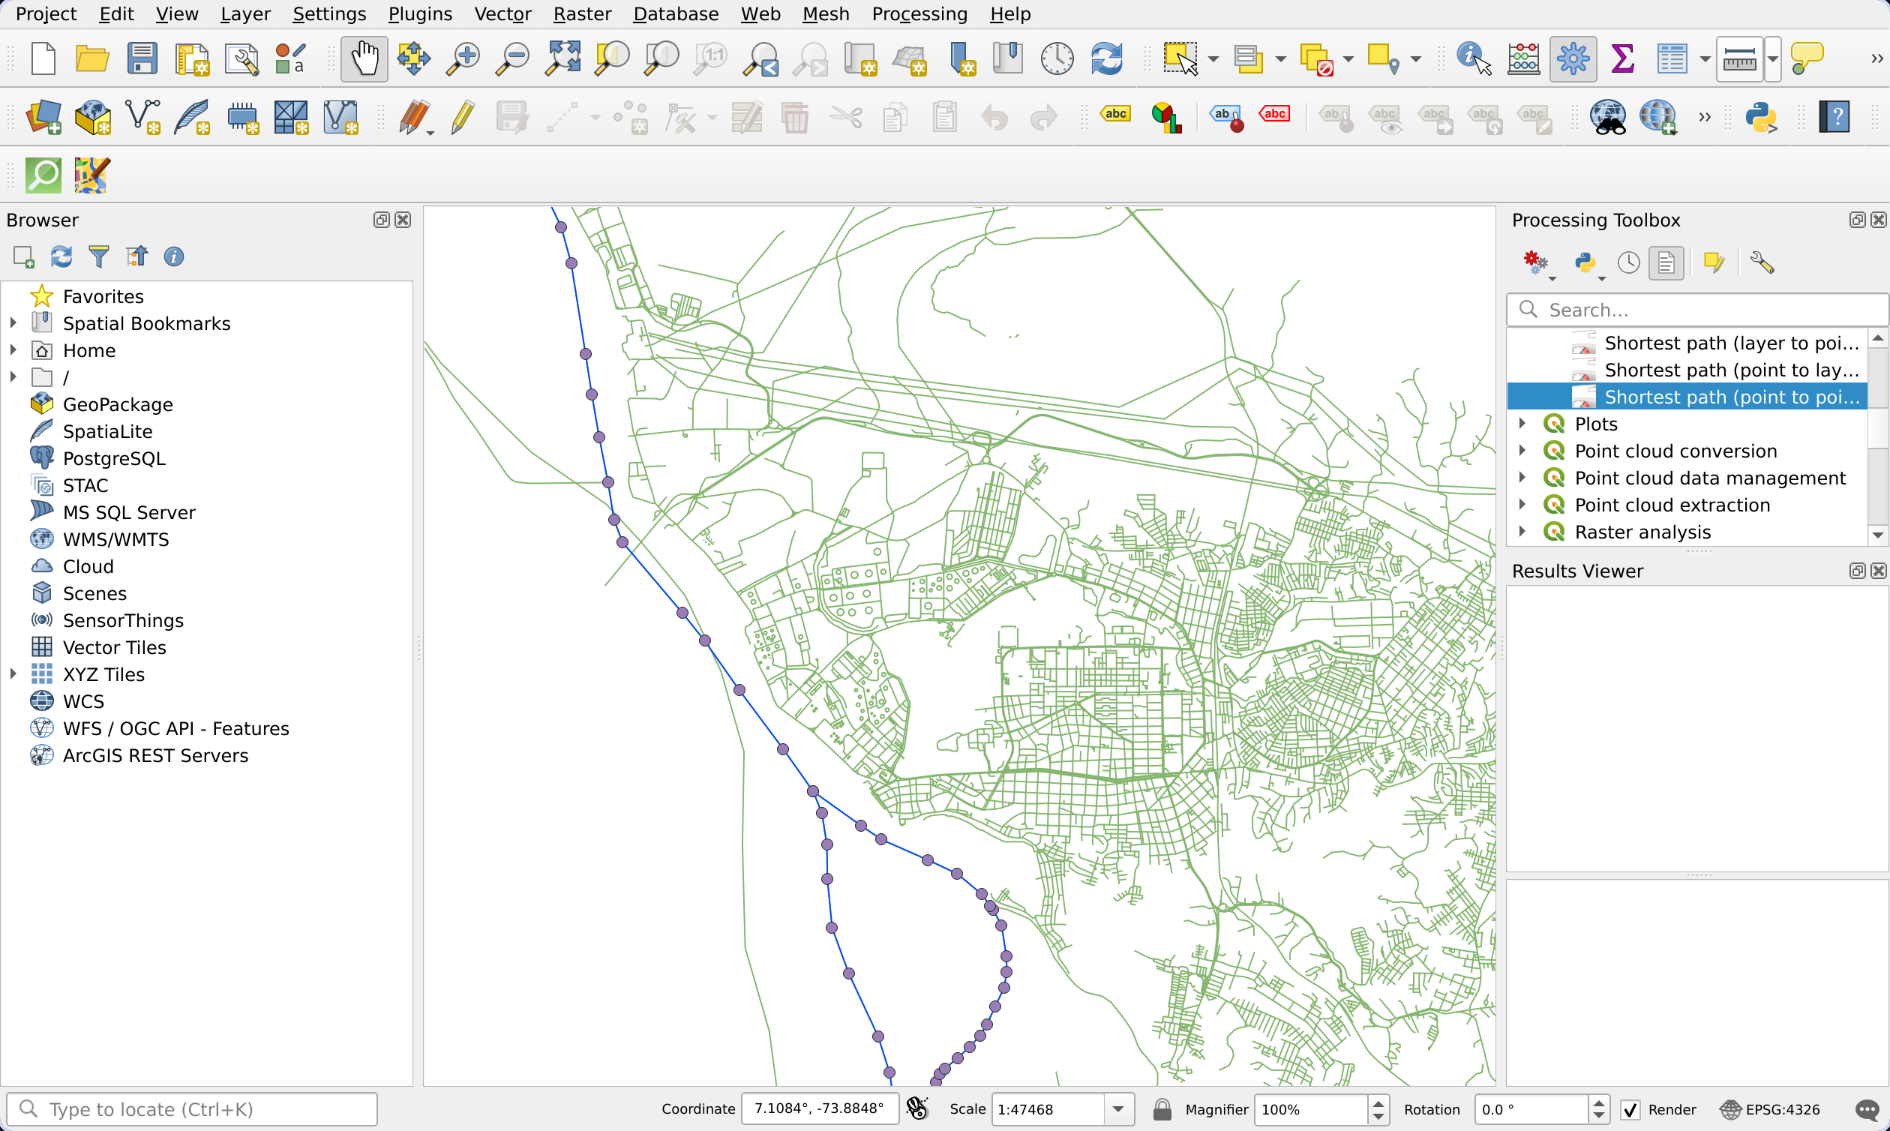
\includegraphics[width=0.8\textwidth]{img/QGIS-3.png}
        \caption{Elaboración propia.}
      \end{figure}
    \end{column}
  \end{columns}

  \begin{columns}
    \begin{column}{.3\textwidth}
      \begin{itemize}
        \item Se seleccionan el segmento que se de interés para el estudio. 
      \end{itemize}
    \end{column}

    \begin{column}{.7\textwidth}
      \begin{figure}[ht]
        \centering
        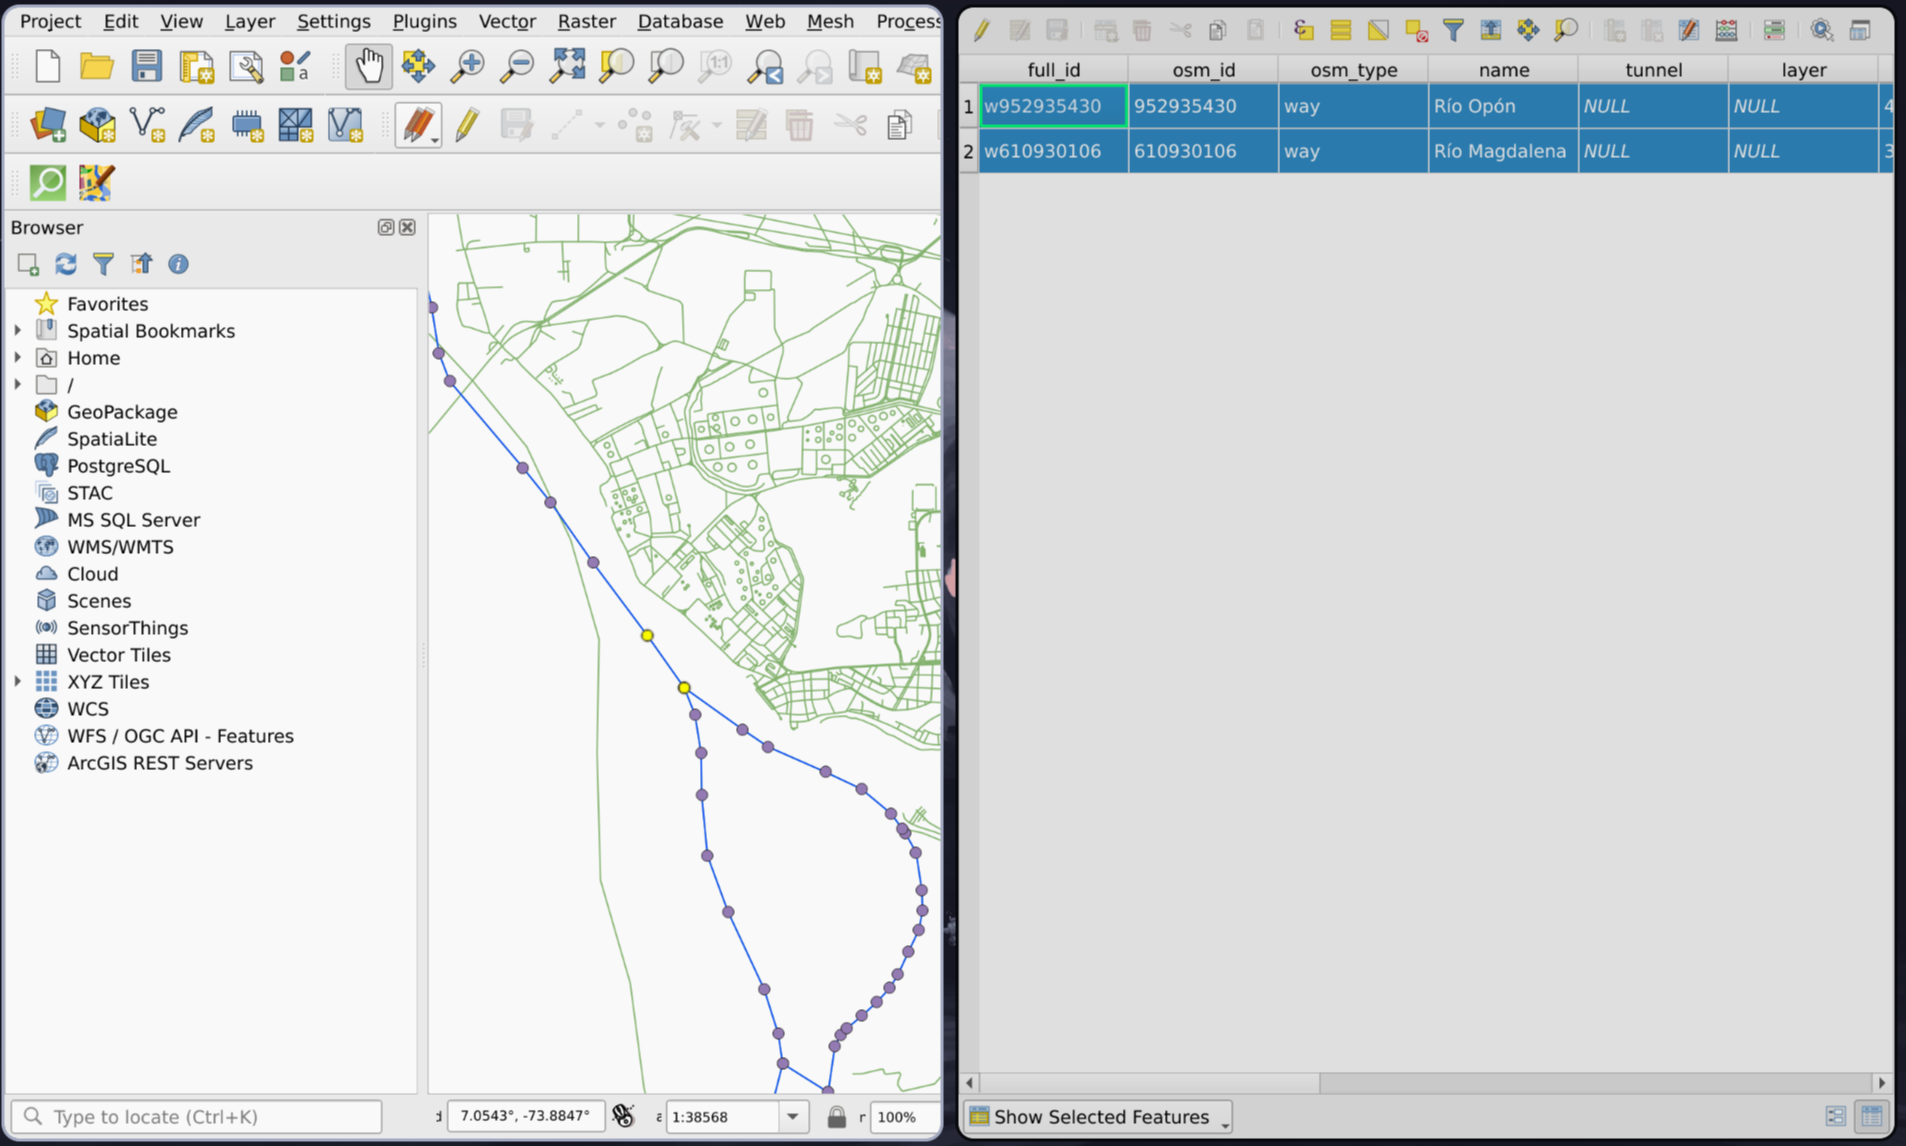
\includegraphics[width=0.8\textwidth]{img/QGIS-4.png}
        \caption{Elaboración propia.}
      \end{figure}
    \end{column}
  \end{columns}

  \begin{columns}
    \begin{column}{.3\textwidth}
      \begin{itemize}
        \item Utilizando la herramienta de \texttt{Distance matrix...} se obtienen $472.7434 \text{ metros}$ .
      \end{itemize}
    \end{column}

    \begin{column}{.7\textwidth}
      \begin{figure}[ht]
        \centering
        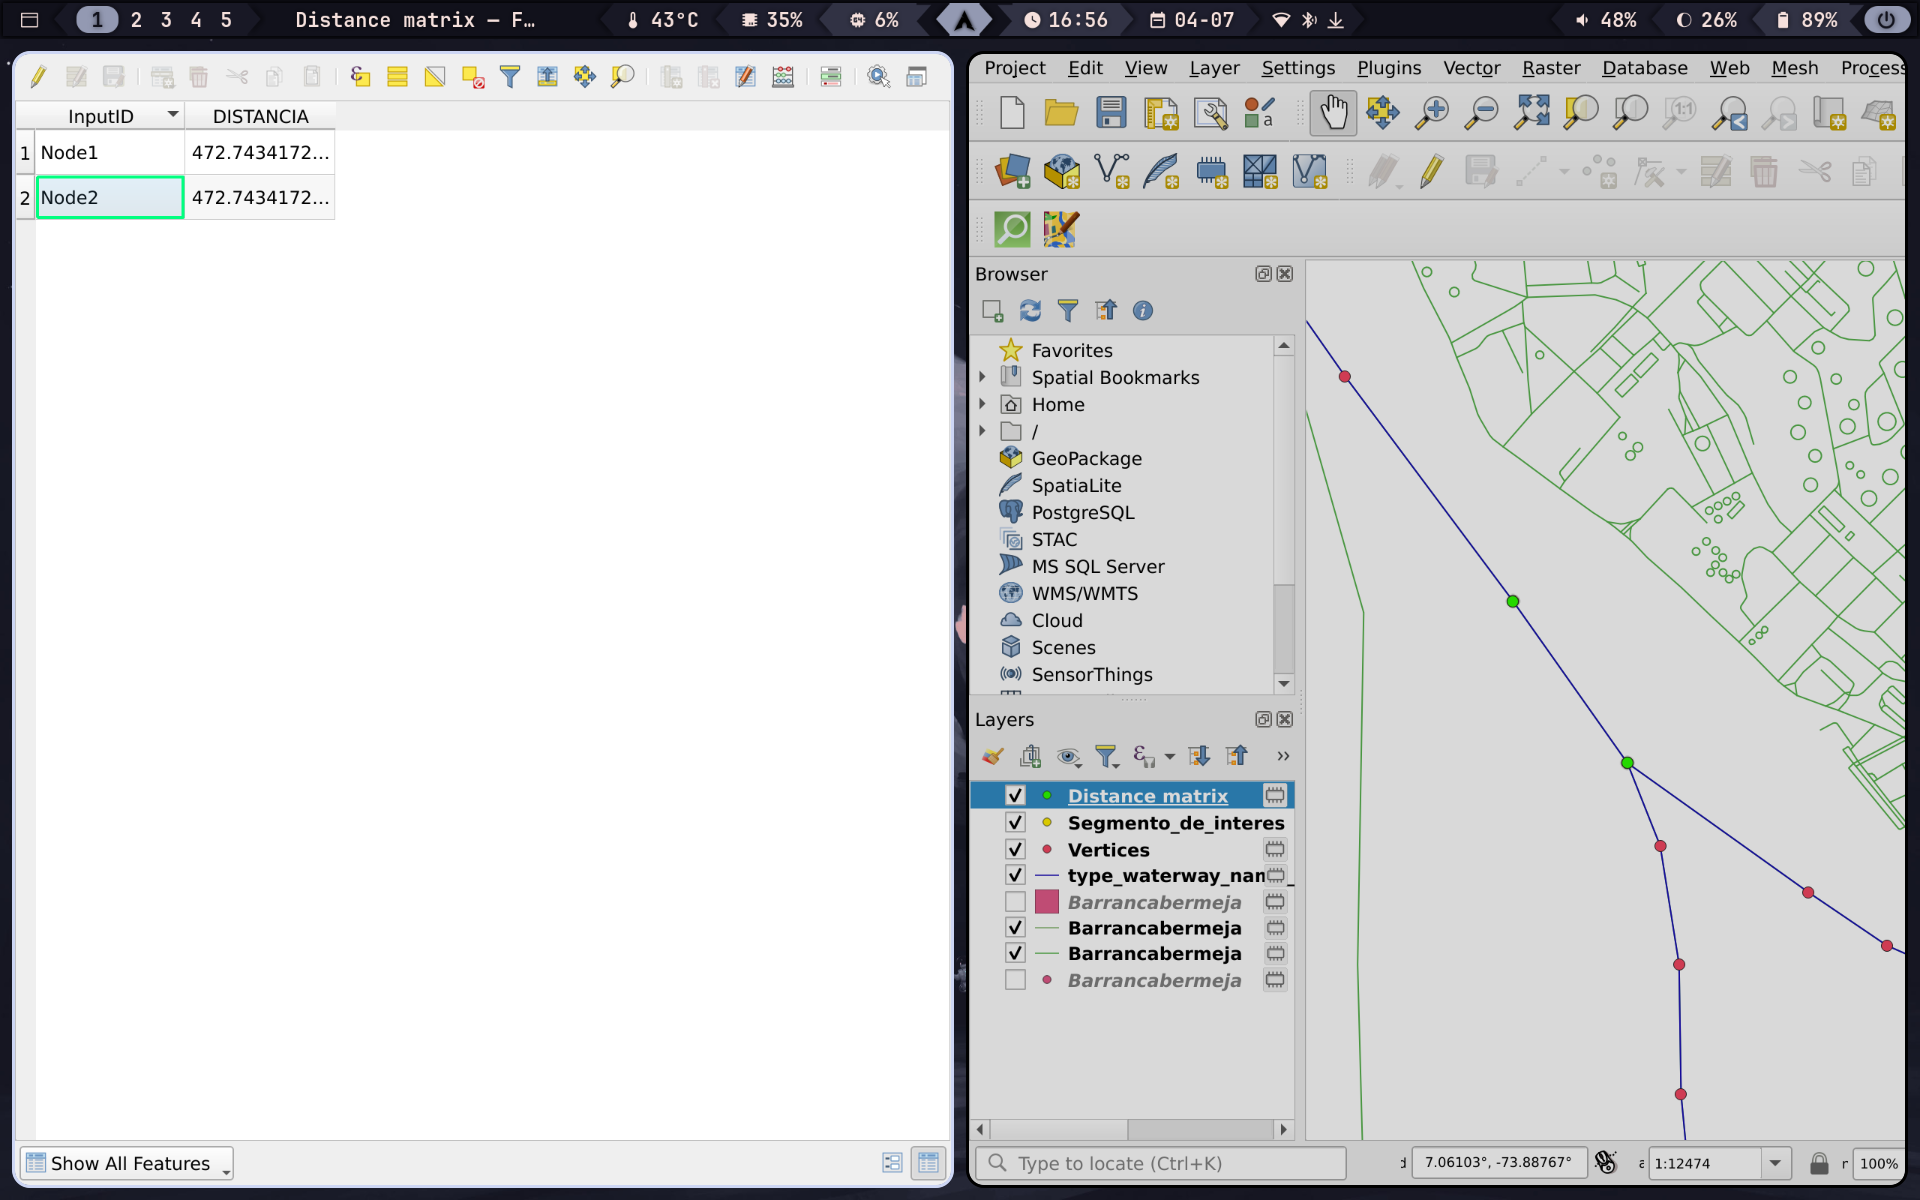
\includegraphics[width=0.7\textwidth]{img/QGIS-6.png}
        \caption{Elaboración propia.}
      \end{figure}
    \end{column}
  \end{columns}

\end{frame}

\begin{frame}
  \frametitle{Consulta del ancho}

  \begin{columns}
    \begin{column}{.3\textwidth}
      \begin{itemize}
        \item Usando la opción \texttt{Open Field Calculator} se puede consultar la información de estos datos como si fuera SQL.
        \item El resultado de esto son $300 \text{ metros}$
      \end{itemize}
    \end{column}

    \begin{column}{.7\textwidth}
      \begin{figure}[ht]
        \centering
        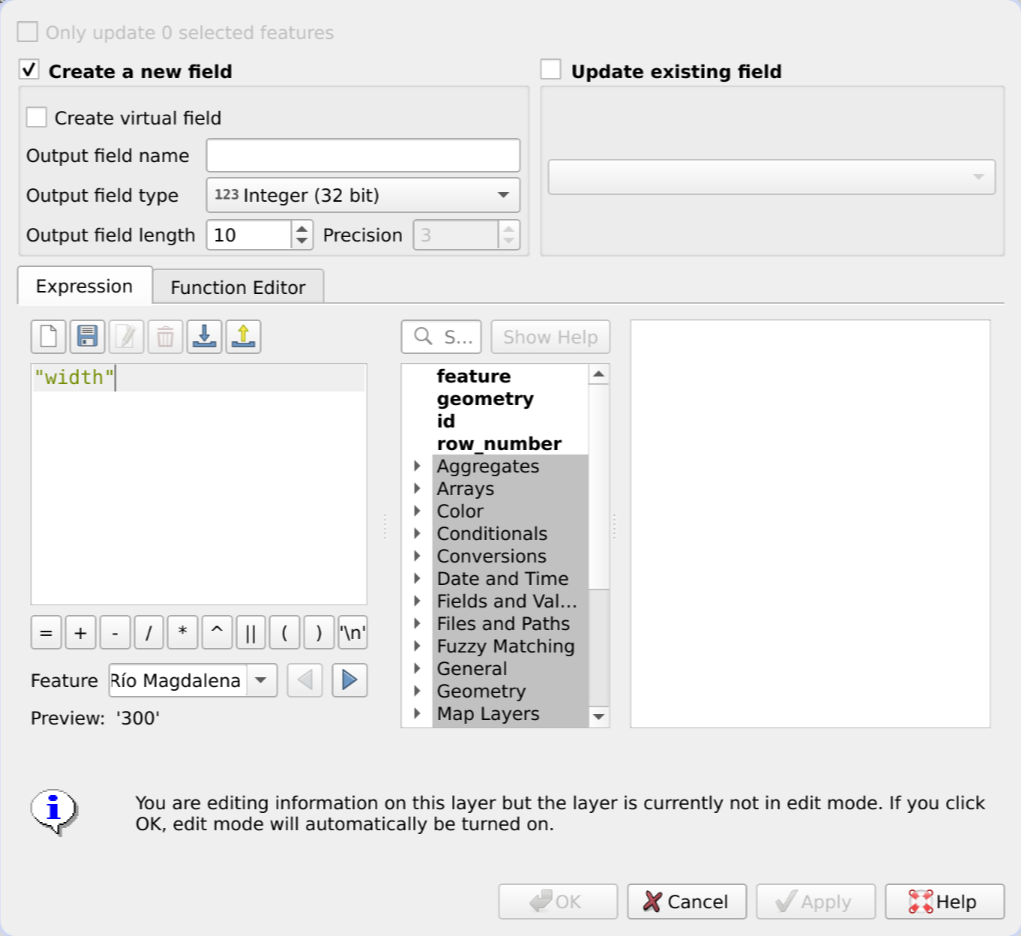
\includegraphics[width=0.5\textwidth]{img/QGIS-7.png}
        \caption{Consulta del ancho del Río Magdalena.}
      \end{figure}
    \end{column}
  \end{columns}

\end{frame}

\begin{frame}
  \frametitle{Coeficiente de rugosidad y pendientes}

  \begin{columns}
    \begin{column}{.3\textwidth}
      \begin{itemize}
        \item Coeficiente de Mannig: $0.018$
        \item Pendiente del río: $0.07\%$
      \end{itemize}
    \end{column}

    \begin{column}{.7\textwidth}
      \begin{figure}[ht]
        \centering
        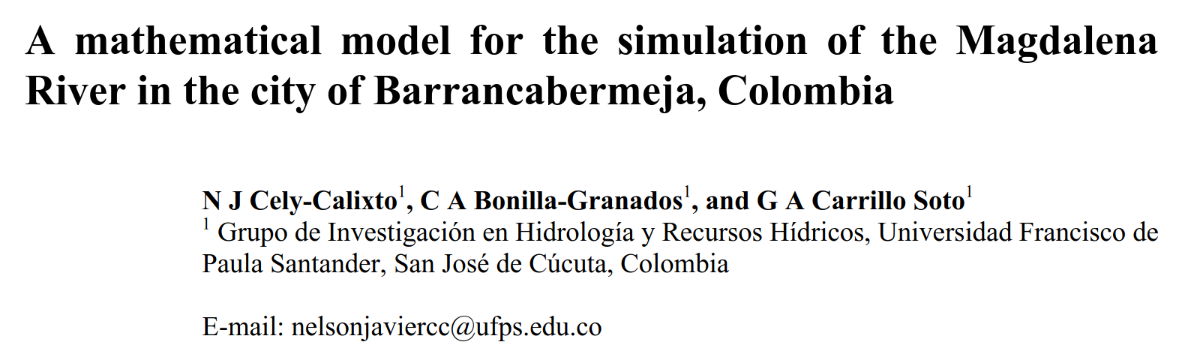
\includegraphics[width=1\textwidth]{img/Paper.png}
        \caption{\textit{A mathematical model for the simulation of the Magdalena River in the city of Barrancabermeja, Colombia}\cite{garcia2020mathematical}.}
      \end{figure}
    \end{column}
  \end{columns}

\end{frame}


\begin{frame}
  \frametitle{Elevación del río}

  \begin{columns}
    \begin{column}{.3\textwidth}
      \begin{itemize}
        \item Script en \textit{Python} utilizando web scrapping con BeautifulSoup
        \item Datos desordenados.
      \end{itemize}
    \end{column}

    \begin{column}{.7\textwidth}
      \begin{figure}[ht]
        \centering
        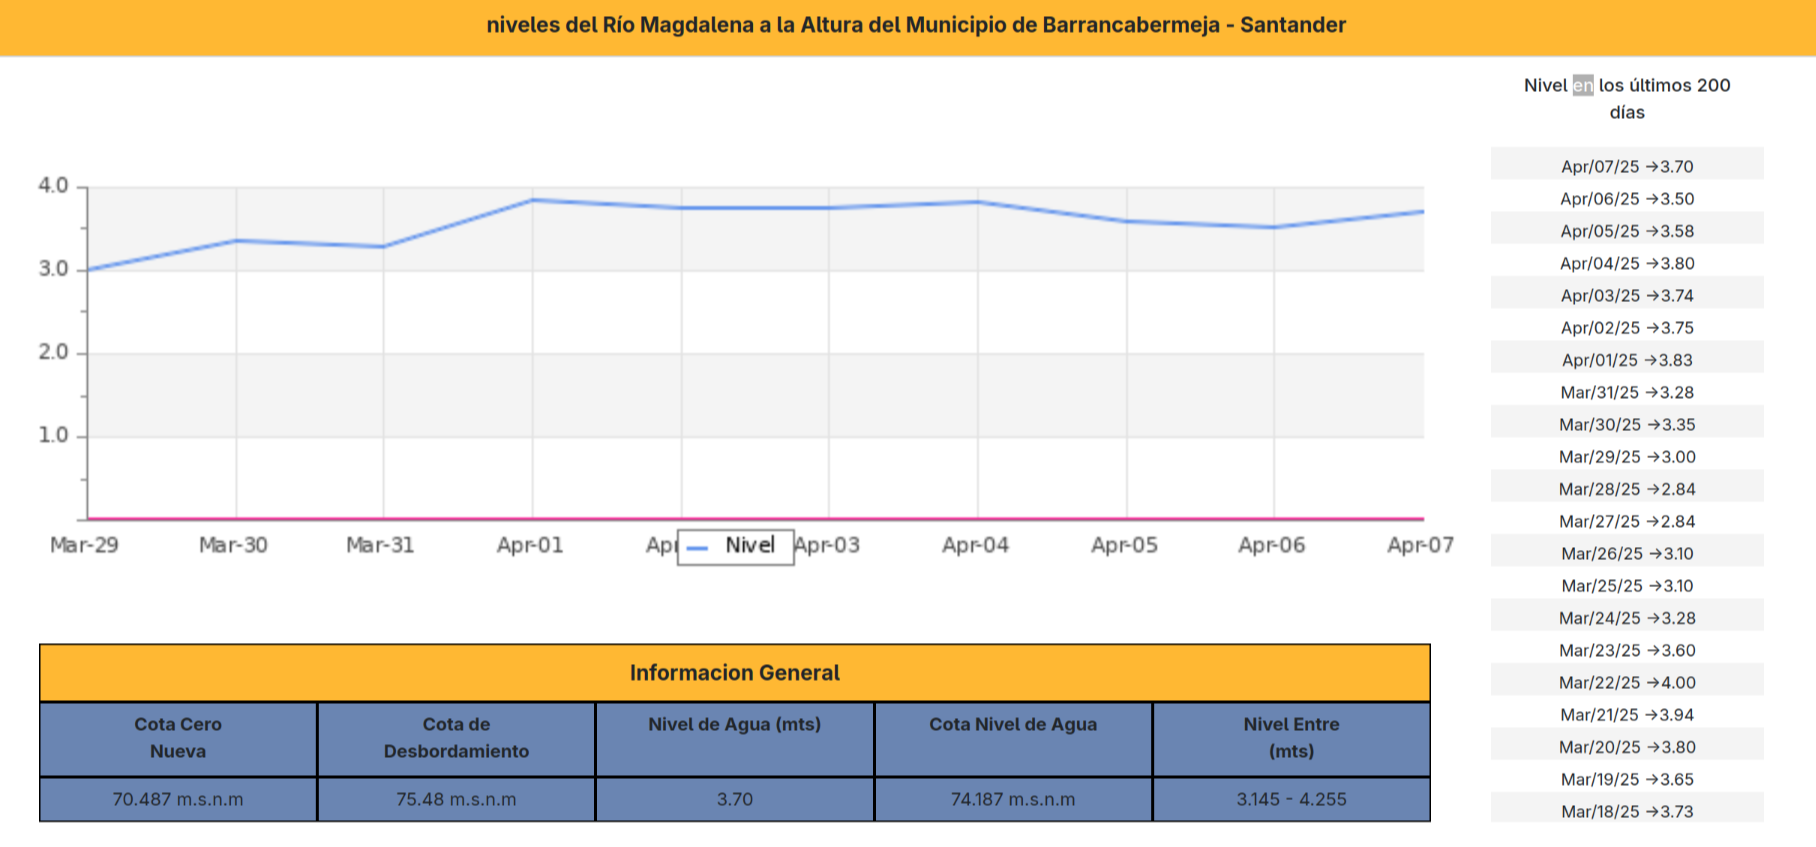
\includegraphics[width=1\textwidth]{img/Barran.png}
        \caption{Datos de CORMAGDALENA\cite{cormagdalena_niveles}}
      \end{figure}
    \end{column}
  \end{columns}

\end{frame}


\section{Modelo matemático}

\insertsectionpage

\begin{frame}
  \frametitle{Ecuaciones de Saint-Venant - Ecuación de continuidad}
  \[
    \frac{\partial s_{c} (A + A_{0})}{\partial t} + \frac{\partial Q}{\partial x} - q_{L} = 0
  \]
  \begin{itemize}
    \item $s_{c}$ es el coeficiente de sinuosidad.
    \item $A$ es el área.
    \item $t$ es el tiempo.
    \item $Q$ es el cauldal.
    \item $x$ es la distancia del río.
    \item $q_{L}$ es el flujo lateral.
  \end{itemize}
\end{frame}

\begin{frame}
  \frametitle{Ecuaciones de Saint-Venant - Ecuación de continuidad}
  \[
  \frac{\partial S_{m}Q}{\partial t} + \frac{\partial (\beta Q^{2} / A) }{\partial x} + g A \left(\frac{\partial h_{r}}{\partial x} + S_{f} + S_{ec}  \right) + M_{L} = 0
  \]
  \begin{columns}
    \begin{column}{0.5\textwidth}
      \begin{itemize}
        \item $S_{m}$ es el factor de sinuosidad.
        \item $Q$ es el caudal.
        \item $t$ es el tiempo.
        \item $\beta$ es el coeficiente del momentum para la distribución de la velocidad.
        \item $A$ es el área.
        \item $x$ es la distancia del río.
      \end{itemize}
    \end{column}

    \begin{column}{0.5\textwidth}
      \begin{itemize}
        \item $g$ es la aceleración de la gravedad.
        \item $h_{r}$ es la altura del río.
        \item $S_{f}$ es la fricción de la pendiente.
        \item $S_{ec}$ es la pérdida por fricción.
        \item $M_{L}$ es el flujo del momento en los bordes.
      \end{itemize}
    \end{column}
  \end{columns}
\end{frame}

\begin{frame}
  \frametitle{Método de diferencias finitas - Ecuación de continuidad}

  \begin{align*}
  &\frac{\partial s_{c} (A + A_{0})}{\partial t} + \frac{\partial Q}{\partial x} - q_{L} = 0 \\
  &\frac{s_{c} (A + A_{0})_{i}^{j+1} - s_{c}(A + A_{0})_{i}^{j} }{\Delta t} + \frac{Q_{i}^{j} - Q_{i-1}^{j} }{\Delta x} - q_{Li}^{j} = 0   
\end{align*}

  \[
  A_{i}^{j+1} = \frac{\left(q_{Li}^{j} - \frac{Q_{i}^{j} - Q_{i-1}^{j} }{\Delta x}  \right) \Delta t + s_{c} (A + A_{0})_{i}^{j}}{s_{c}} - (A_{0})_{i}^{j+1}
  \]
  
\end{frame}


\begin{frame}
  \frametitle{Método de diferencias finitas - Ecuación de momentum}

  \begin{align*}
  \frac{s_{m} (Q)_{i}^{j+1} - s_{m}(Q)_{i}^{j} }{\Delta t} + \frac{(\beta Q^{2}/A)_{i}^{j} - (\beta Q^{2} /A)_{i-1}^{j} }{\Delta x} + gA \left( \frac{(h_{r})_{i}^{j} - (h_{r})_{i-1}^{j}}{\Delta x} + S_{f} + S_{ec}   \right) + M_{L} = 0   
\end{align*}

  \[
  Q_{i}^{j+1} = \frac{\left[ -M_{L} - g(A_{i}^{j}) \left(\frac{\left(\frac{A}{W}\right)_{i}^{j} - \left(\frac{A}{W}\right)_{i-1}^{j} }{\Delta x} + S_{t} + S_{a}  \right) - \frac{ \left( \frac{\beta Q^{2}}{A} \right)_{i}^{j} - \left( \frac{\beta Q^{2}}{A} \right)_{i-1}^{j}  }{\Delta x}           \right] \Delta t + S_{m} (Q)_{i}^{j}}{s_{m}}
  \]
  
  
\end{frame}


\begin{frame}
  \frametitle{Más modelos}

  \begin{itemize}
    \item Preissman por 4 puntos.
    \item Método de características.
    \item Método de elementos finitos.
    \item Las ecuaciones no tienen solución analítica (excepto en algunos casos).\cite{deaton1999dynamic}
  \end{itemize}
  
\end{frame}


   



\begin{frame}
  \frametitle{Licencia}

  \begin{columns}
    \begin{column}{.5\textwidth}
      \begin{itemize}
        \item Código, datos y contenido se encuentra en: \url{https://github.com/TheLudway/HydrologyDynamicsProject} 
        \item Todo bajo la licencia GPL V3 y CC BY SA 4.0 a excepción de los datos.
      \end{itemize}
    \end{column}

    \begin{column}{.5\textwidth}
      \begin{figure}[ht]
        \centering
        \includesvg[width=0.8\textwidth]{img/GPL.svg}
      \end{figure}
    \end{column}
  \end{columns}

\end{frame}


\section{Referencias}

\insertsectionpage
\begin{frame}[allowframebreaks]{Referencias}
  \printbibliography
\end{frame}


\insertendpage

\end{document}
